\newpage
%%%%%%%%%%%%%%%%%%%%
\section{Animations}
\label{sec:animations}

Sudden and unexpected changes in a user interface, e.g., objects moving from one position to another without any transition between the two states, put a heavy cognitive load on the user, who must mentally relate the states in order to re-assimilate the new display \cite{Chang93}. Animating changes applied to user interface objects transfers part of the user effort to the perceptual level, freeing cognitive processing capacity for application tasks \cite{robertson93}. Aside from the aesthetically pleasant impression it produces on most users when used appropriately, animation therefore contributes to make interfaces more user-friendly.

Animations have been used for didactic purposes, for instance to explain algorithms (see e.g. \cite{carlson96, rodgers00}), but tend to be used more and more just for their above-mentioned ability to reduce the user's cognitive load. For instance, desktop animations are ubiquitous in Apple's Mac OS X and contribute to the perceived quality of this operating system's GUI. Closer to our domain, many information visualization toolkits also support some animation primitives often centered on objects' position. Other toolkits \cite{Chang93, hudson93,bederson00,bederson04} provide more advanced animation support.

ZVTM offers animation capabilities inspired by Stasko's path/transition paradigm \cite{stasko90}. Many user interface changes can be animated following a unified declarative API. Variables to which animations can be applied include:
\begin{itemize}
\item all basic glyph variables (position, orientation, size, color and translucency) and control points of curves (DPath);
\item camera translations and altitude changes (zoom-in/out);
\item magnification lens' radii and magnification factor modifications;
\item portals' location within a view, their size, and translucence.
\end{itemize}

\begin{figure}[!ht]
\centering
 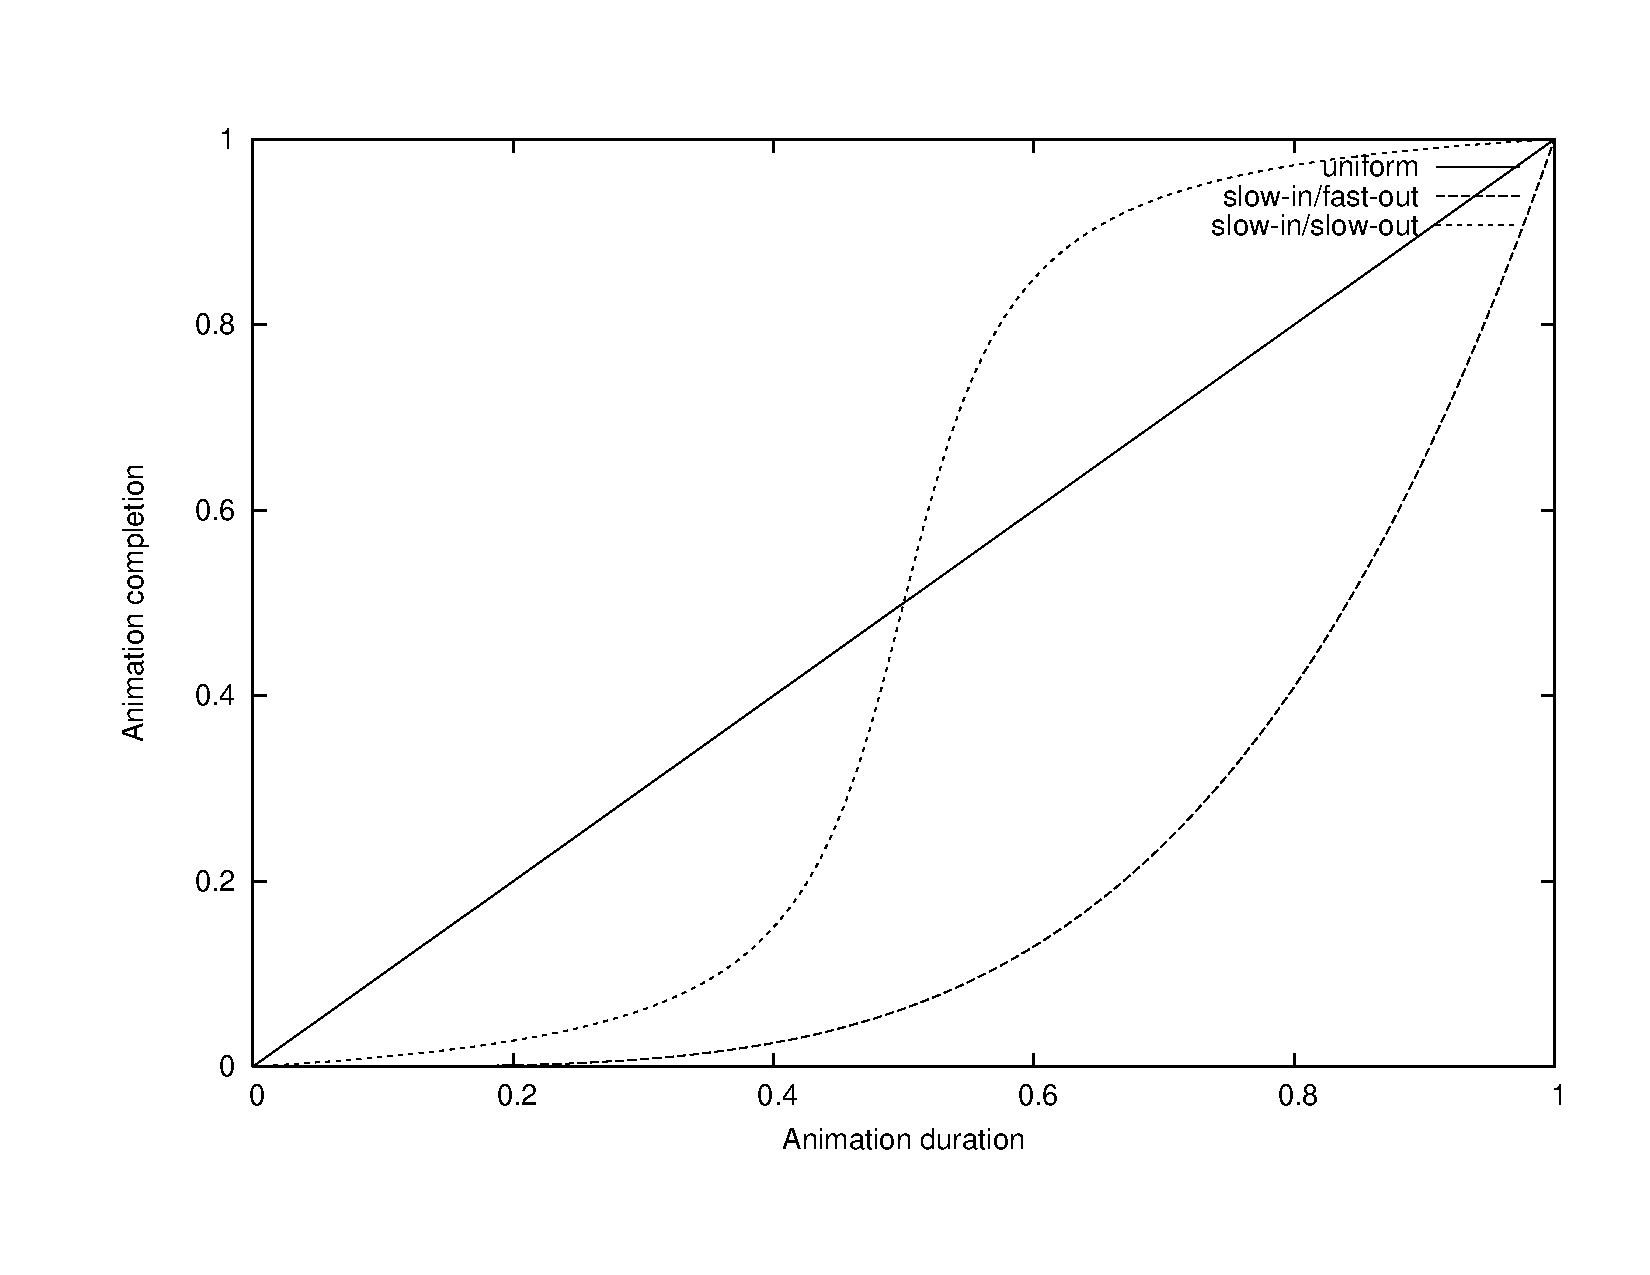
\includegraphics[width=16cm]{images/animSchem.pdf}
  \includegraphics[width=5.5cm,angle=-90]{images/animSchemEx.pdf}
   \caption{Animation pacing functions (top) and example on the translation of a rectangle (bottom)}
   \label{fig:pacing}
\end{figure}

Animations are specified with a single instruction and do not require much more code than the basic modification of a variable's value. They require the following parameters: the animation duration, the object involved, the variable(s) impacted by the animation, the desired target value, and the pacing function. Three off-the-shelf pacing functions are available (Figure \ref{fig:pacing}). Slow-in/slow-out transitions are typically used for camera motion and some glyph animations such as translations, as they convey a feeling of solidity that is important in direct manipulation interfaces \cite{Chang93}. Non-uniform pacing functions are generally used to put emphasis on the start (and/or end) of animation paths. However, they are not always appropriate, and the uniform function is often used when modifying, e.g., magnification lens parameters, or when animating color changes.

Animations are managed by a dedicated thread that controls their timing precisely, skipping steps on the computed animation path if necessary. This mechanism ensures that an animation lasts the specified duration, and runs as smoothly as the system and hardware performance allow. Until v0.9.7, ZVTM was using its own animation engine. Since v0.10.0, the animation engine has been completely rewritten and is now based on Sun's Timing Framework\fref{https://timingframework.dev.java.net/}, and now features additional capabilities in terms of animation management. The use of this more generic API should also make it easy for people already familiar with the Timing Framework to write animations in ZVTM. We only describe the new API in the following.

\subsection{Animation Module: Overview}
The Animation module in ZVTM is heavily based upon the Timing Framework (it can be seen
as a subset of the Timing Framework augmented with convenience functions).

From this framework, we borrow the concepts of Timing Sources, Interpolators and Timing Targets 
(called Timing Handlers in our API). 
We discard the idea of an Animator targetting multiple receivers in favor of an Animation class
that animates a single object (Glyph, Camera, Portal, Lens or Translucent).


\subsection{The Animation Object}
The Animation object encapsulates an animation that has a single target and dimension.
Dimensions are enumerated in the \cd{Animation.Dimension} enum.

\subsection{Creating an Animation: the Flexible Way}
The generic way to create an Animation is to use one of the three createAnimation() methods
of AnimationFactory. We will examine the most generic one, since the other two are simply
overloads that provide defaults. Here is an example:

\begin{SaveVerbatim}{CodeVerb}
Animation cameraAlt = am.getAnimationFactory().createAnimation(
   4000, 
   2f,
   Animator.RepeatBehavior.REVERSE,
   vsm.getVirtualSpace("src").getCamera(0),
   Animation.Dimension.ALTITUDE,
   new DefaultTimingHandler(){
      public void timingEvent(float fraction, 
                                            Object subject, 
                                            Animation.Dimension dim){
         Camera c = (Camera)subject;
         c.setAltitude(25+Float.valueOf(fraction*50).longValue());
   }
                                             
      public void end(Object subject, Animation.Dimension dim){
         circle2.setColor(Color.RED);
      }
   },
   ConstantAccInterpolator.getInstance()
);
\end{SaveVerbatim}
\fbox{\BUseVerbatim[boxwidth=0.99\columnwidth]{CodeVerb}}


\subsection{Creating an Animation: the Easy Way}
Ready-made Animation factory methods are provided as a convenience, to cover the most common
cases. These are part of the \cd{AnimationFactory} class. 
These factories are named create[TargetType][AnimationType].
For instance, a Glyph translation can be created by calling 

\codebox{vsm.getAnimationManager().getAnimationFactory().createGlyphTranslation(...);}

(where \cd{vsm} is a reference to your application's \cd{VirtualSpaceManager})

\subsection{Controlling Animations}
Animations are controlled from the AnimationManager.
There is a unique animation manager per VirtualSpaceManager.
Once created, animations need to be started to start taking effect.
Animations will automatically stop after their programmed duration, but it is possible
to force an animation to stop early or cancel it completely.

\subsubsection{The Queue System}
Animations have a dimension property and a subject (the object being animated).
Two animations are said to conflict if they target the same subject \emph{and} have the same dimension.
Conflicting animations are executed in sequence, while orthogonal animations (those that do not conflict)
are executed concurrently.

Conceptually, you can think of the queue system as a number of queues: one queue for each
(subject, dimension) pair (although they are not implemented in that way). 
Animations are put into those queues by calling AnimationManager.startAnimation().
The first animation of the queue is running, and will leave the queue upon completion, 
where if it will be replaced by the next animation in line (if it exists).
  
\subsubsection{Starting an Animation}
Suppose that you have a reference \cd{anim} to an Animation that was created using the AnimationManager factory,
you may start it by calling

\codebox{am.startAnimation(anim, false)}

The boolean parameter will put \cd{anim} in the queue in the normal fashion if set to false,
or cancel all conflicting animations prior to enqueing \cd{anim} if set to true, thus
ensuring that the animation will start immediately. 
  
\subsubsection{Stopping or Cancelling an Animation}
If you want an animation to end without waiting for completion, you may use the
AnimationManager \cd{stopAnimation} and \cd{cancelAnimation} methods.
Both take a single parameter: a reference to the \cd{Animation} that must be stopped or cancelled.
The difference between stopping and cancelling an Animation is that the end action (\cd{end} method
of a \cd{TimingHandler} or \cd{execute} method of an \cd{EndAction} will be executed if the animation
is stopped, but not if it is cancelled.

\subsubsection{Pausing and Resuming an Animation}
In addition to starting, stopping and cancelling Animations, it is possible to put them on hold.
This feature is seldom used in practice. 

  
